\documentclass[11pt]{article}
\usepackage[margin=2.54cm]{geometry}
\usepackage[colorlinks,urlcolor=blue]{hyperref}
\usepackage{url}
\usepackage{graphicx}

\title{Classifying Movie Genres With Plot Summaries}
\author{Brian Kimmig, Jesus Zarate}
\date{}

\begin{document}

\maketitle


\section{Introduction}
\label{sec:introduction}

The internet today contains an abundance of information. We see a great deal of images, videos, and somewhat more common, text. It is common that people want to summarize a topic or the content of a chunk of text. This is a challenging problem for computers and machine learning (ML) algorithms as sentences and paragraphs are highly unstructured. A majority of ML algorithms require the data to be in a consistent form, from vectors to matrices. Furthermore, they require that the data is numerical. This poses the main problem for us, how do you meaningfully turn a sentence or paragraph into numerical data?

The goal of this project was to take text data, and assign it to a category (or categories). We could try to do this with Twitter data but the categorizing of Tweets can be largely subjective and was beyond the scope of this class. We decided that a good dataset to try these methods on would be film synopses and genres. In this case the the text describing a movie can vary greatly, but there is a consistent and widely agreed on genre categorization. This makes for a great dataset to help us see if we can categorize textual data. We aim to see if we can take the text of a film synopses, build meaningful features, and learn a model to categorize the genres of other movies based on their synopses. 

% TODO
Building meaningful features from text sounds nice, but what does that actually mean? Go into other stuff here? What methods are we planning on using? Point to them below?
 
\section{Data}
\label{sec:data}

We obtained the base of our data from a dataset published on \href{https://www.kaggle.com/deepmatrix/imdb-5000-movie-dataset}{Kaggle}. The dataset contained information on $\sim5000$ movies. We used this dataset for the movie list and the IMDB IDs. With IMDB IDs it is easy to automate gathering the synopses of each movie via GET requests to the \href{https://www.omdbapi.com/}{OMDB API}. The OMDB API allows you to search for movies, and gather information via the title or the IMDB ID. To ensure we get the correct information for every movie we performed GET requests querying with the IMDB ID. 

The OMDB API allows a user to specify the length of the plot summary it returns, with either 'full' or 'short'. We chose to gather the 'full' synopses for every movie we queried.

From the Kaggle data we used the OMDB API to compile title, plot summary, and genres for all $\sim5000$ movies. The data was stored in a JSON file, with each entry (or movie) containing the fields ['title', 'plot', 'genres'].

There were considerably more genres than expected, in total there were 26. Figure \ref{fig:genres} shows every genre and its percent occurrence. In our data, there were genres that occurred less than 1\% of the time, and generally they tended to be more obscure genres. Specifically, the genre 'Game-Show' occurred 0.02\% of the time. Because of the rare genres we decided to limit our genre classification labels to those that occur more often. In the end we settled on a cut of 5\% (shown by the red dotted line in Figure \ref{fig:genres}). This was to ensure that we had captured the major, or most common, genres. The cut of 5\% also allowed us to ensure that every movie had at least 1 label, or genre, associated with it. If the cut was higher, we found that some movies did not have a genre associated with it. We also wanted to avoid throwing away data. 

\begin{figure}[ht]
	\centering
		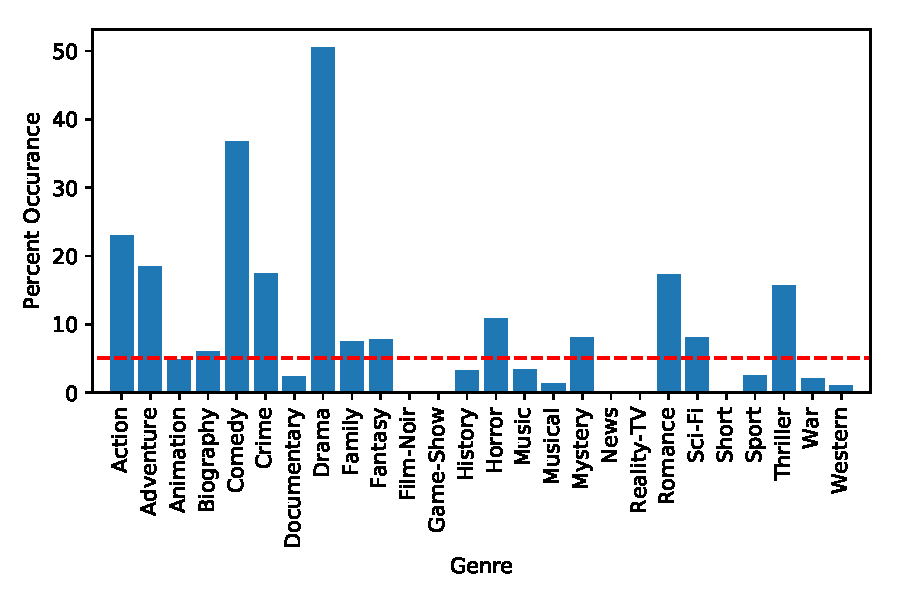
\includegraphics[width=0.75\textwidth]{genres.pdf}
	\caption{The percent occurrence for each genre. The red dotted line represents the cut made to get the list of genres (5\%).}
	\label{fig:genres}
\end{figure}

In the end, with our 5\% cut we ended up with the genres Action, Adventure, Comedy, Crime, Drama, Romance, and Thriller.

The genre labels set up with a one hot encoding. This was done to allow us to easily classify them with either a multi label classifier, or by individually, by column, with other classifiers (discussed further in \S \ref{sec:methods}). Figure \ref{fig:one_hot} shows the genres for every movie in the one hot encoding. A yellow line indicates the movie is associated with that genre, from this we can clearly see that a majority of the movies are associated with the 'Drama' genre.

\begin{figure}[ht]
	\centering
		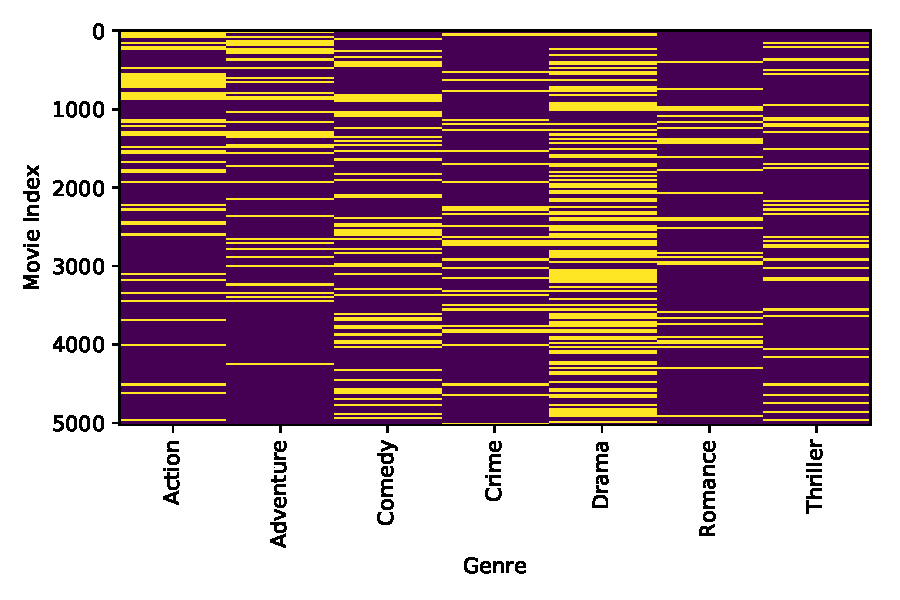
\includegraphics[width=0.75\textwidth]{one_hot_genres.pdf}
	\caption{The one hot encoding of the genres for every movie. Each row represents a movie and a column represents a genre. Yellow indicates the movie has that genres associated with it.}
	\label{fig:one_hot}
\end{figure}

The synopses of the movies live in long strings or documents. We have a list of these that we will processing to create the features that we will then use to build models to classify genres. Extracting features from these documents is the main part of the project and will be discussed \S \ref{sec:methods}.

\section{Methods and Results}
\label{sec:methods}

In this section we will discuss the methods we used to create features for classification. We will start by creating features using Term Frequency - Inverse Document Frequency (TF-IDF), then with Latent Dirichlet Allocation \cite{blei2003}, and finally a combination of the two. 

We will classify genres of movies with three different classifiers. The first will be a simple linear regression, as learned in class. The labels are binary for each genre, so some thresholding will be done to get labels using linear regression. Next, we will classify with logistic regression, which is a well known regression model for predicting binary labels. For both linear and logistic regression we will fit for each genre individually. The last classifier we use will be the random forest \cite{breiman2001}. We chose to use Random Forests due to their popularity in data science competitions and their multi label classification capabilities; we can classify all labels simultaneously. 

For both the logistic regression, and random forest classifier we used the scikit-learn implementations \cite{scikit-learn}.

\subsection{Term Frequency - Inverse Document Frequency}
\label{sec:tfidf}

\subsubsection{Linear Regression}

Classify one genre at a time.

\subsubsection{Logistic Regression}

Classify one genre at a time.

\subsubsection{Random Forrest}

Classify all genres at once.


\subsection{Latent Dirichlet Allocation}
\label{sec:lda}

Topic models are methods of taking large amounts of data and finding, understanding, and summarizing the information in it \cite{wiki:topic_model, kdnuggets:topic_model}. We believe that hidden in these plot summaries there will be some fairly obvious groups of words, or topics, that will be seen together. After some on-line research we came across the concept of Latent Dirichlet Allocation (LDA) \cite{blei2003}. LDA is a fairly popular topic model. 

LDA essentially looks for topics in documents, determines some topics, and gives an estimate of the proportion of that topic that is seen in the document. The general idea that documents are random mixtures of topics, and topics are characterized by words \cite{blei2003}. 

\subsubsection{Linear Regression}

\subsubsection{Logistic Regression}

\subsubsection{Random Forrest}

\subsection{TF-IDF + LDA}
\label{sec:tfidf_lda}

\subsubsection{Linear Regression}

\subsubsection{Logistic Regression}

\subsubsection{Random Forrest}

\section{Discussion}
\label{sec:discussion}

\subsection{Brian's Thoughts}

\subsection{Chuy's Thoughts}

\bibliography{bibliography}{}
\bibliographystyle{plain}

\end{document}

% \begin{table}[h]
% 	\label{tab:genres}
% \begin{center}
% 	\begin{tabular}{| l | l |}
% 		\hline
% 		Genre & \% Occurrence \\
% 		\hline
% 		Action & 23.007\% \\
% 	  \hline  
% 	\end{tabular}
% \end{center}
% 	\caption{}
% \end{table}
